\documentclass{article}

\usepackage[T1]{fontenc}
\usepackage[utf8]{inputenc}
\usepackage[english, danish]{babel}
\usepackage{parskip}
\usepackage{fancyhdr}
\usepackage[outputdir=.]{minted}
\usepackage{float}
\usepackage{graphicx}
\usepackage{caption}
\usepackage{hyperref}
\usepackage{cleveref}
\usepackage{csquotes}
\usepackage[style=ieee]{biblatex}
 
\newcommand{\source}[1]{\caption*{\hfill Kilde: {#1}} }
\newcommand\fnurl[2]{\href{#2}{#1}\footnote{\url{#2}}}

\addbibresource{references.bib}

\setcounter{secnumdepth}{6}
\pagestyle{fancy}
\fancyhf{}
\rhead{UCL Vejle, Pba. i Softwareudvikling}
\lhead{Simon Bo Dall Mikkelsen}
\rfoot{Side \thepage}

\begin{document}

\title{Test af Microservice Baserede Systemer}
\author{Simon Bo Dall Mikkelsen \\ \href{mailto:simo451g@edu.eal.dk}{simo451g@edu.eal.dk}}
\date{\today}

\maketitle
\thispagestyle{empty}
\newpage

\tableofcontents
\thispagestyle{empty}
\newpage

\section{Problemformulering}

Microservice arkitekturen er blevet et populært alternativt valg til monolistiske applikationer, for software systemer af større størrelser, men \emph{hvordan kan et sådan system bedst muligt testes?}

Problemstillinger:

\begin{enumerate}
    \item Hvordan testes en microservice? \ref{sec:how-to-test-a-microservice}
    \item Hvordan testes sammenspillet mellem microservices? \ref{sec:how-to-test-microservice-collaboration}
\end{enumerate}

\section{Uddybning}

\paragraph{Hvordan testes en microservice?}\label{sec:how-to-test-a-microservice}

Software systemer har klassisk været struktureret som enlige monolitter. Disse følger oftest klar lagdeling, men ikke konkret modulisering af funktionalitet. Mens ikke designet omkring den monolitiske struktur, bliver de klassiske test teknikker oftest fremvist i denne sammenhæng. 

En microservice kan i praksis anses for, at være en enlig monolit, med et meget mere rafineret forretningsområde, modsat den klassiske monolit, hvilken håndterer alle forretningsområder for systemet selv. Microservice arkitekturen kan siges, at påtvinge den manglende modulisering i den klassiske monolit tilgang, hvor selvstændige forretningsområder separeres ud i egne microservices, hvilke arbejder sammen om, at løse konkrete forretningsopgaver.

Hvordan en typisk monolitisk applikation testes, afspejles derfor delvist i, hvordan en enlig microservice kan testes, dog med nogle ekstra omstændigheder der skal tages højde for.

\begin{figure}[H]
    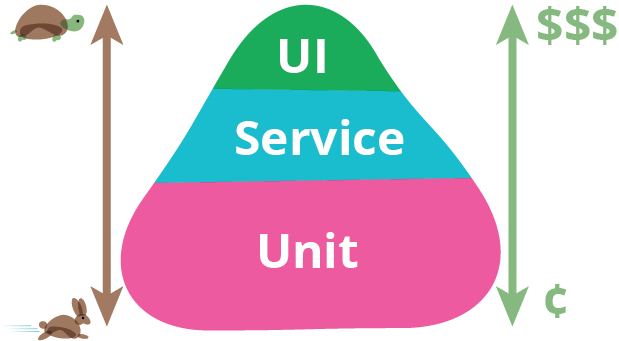
\includegraphics[width=\textwidth]{images/test-pyramid.png}
    \caption{Test pyramiden}
    \source{\cite{fowler:test-pyramid}}
    \label{fig:test-pyramid}
\end{figure}

Test pyramiden set i \cref{fig:test-pyramid}, er en klassisk måde, at visualisere de forskellige former for automatiserede test. Dens essentielle pointe er, at der bør udføres mange flere "low level" test af underliggende individuelle enheder i programmet, end "high level" test af systemet som en helhed. I praksis svarer dette til, at størstedelen af test dækningen sker gennem unit testing, med mindre fokus des tættere man kommer på end-to-end testing.

Når det kommer til best practices indenfor unit testing, benyttes hvad mange kalder for FIRST principperne som kvalitetstjek.

\begin{description}
    \item[Fast] En unit tests eksekveringstid skal være så absolut minimal som mulig, dette inkluderer opsætning samt nedrivning af testen.
    \item[Isolated/independant] En unit test skal være fuldt ud uafhængig af resten af test miljøt. Den følger "3A" strukturen: Arrange, Act, Assert. Den opsætter sin egen nødvendige tilstand. Den fokuserer på en specifik case. Den skal kunne køres uafhængigt, før eller efter en hvilken som helst anden test.
    \item[Repeatable] En unit test er deterministisk og afhænger ikke af nogen antaget tilstand. Den skal rydde op efter sig selv, således den ikke efterlader nogle tilstandsændringer. Den afhænger aldrig af eksterne ressourcer, hvilke ikke nødvendigvis altid er tilgængelige.
    \item[Self-validating] En unit test vil resultere i enten success eller fejl således, at der aldrig behøves konkret tjek af dets resultat.
    \item[Thorough] En unit test bør dække alle scenarier og ikke blot gå efter 100\% kode dækning. Den køres med mange forskellige tilstande. Den køres med alle grænseværdier.
\end{description}

FIRST principperne garanterer, at systemets unit tests vil være tilstrækkeligt dækkende samt, at de med lethed kan automatiseres.

Før der dog overhovedet kan skrives programmatiske unit tests, skal systemets underliggende programkode skrives på en testbar måde. En unit test skal, ifølge FIRST, blandt andet være så isoleret og specifik som muligt. I praksis har dette den betydning, at den enhed en unit test tester, skal have et klart defineret ansvar, med klart definerede afhængigheder. SOLID principperne\footcite{martin:solid}, hvis fulgt korrekt, garanterer som minimum disse kvaliteter og mange flere, der er relevante for testbar kode generelt.

En definerende karakteristik ved en microservice er, at den kommunikerer med andre microservices for, at tilbyde dens fulde funktionalitet. Når en enhed testes i en unit test kontekst, ville denne kommunikation med andre microservices altid mockes, på baggrund af FIRST og gjort muligt af SOLID. At teste den indre funktionalitet af en microservice i isolation fra andre microservices gennem unit tests, garanterer derfor ikke, at kommunikationen mellem microservices fungerer korrekt.

Til at teste kommunikationen mellem microservices, benyttes integration testing. Martin Fowler beskriver integration tests opgave som værende at ``...determine if independently developed units of software work correctly when they are connected to each other.'' \footcite{fowler:integration-test} med den anderkendelse at ``The term has become blurred even by the diffuse standards of the software industry.'' \footcite{fowler:integration-test} 

Integration testing i forbindelse med microservices, er netop en af grundende til, at Fowler indrømmer termets lidt slørrede mening. Her benyttes integration tests nemlig til, at validere en microservices kommunikation med eksterne komponenter, såsom andre microservices, eksterne databaser eller caching services.

Grunden til den lidt utraditionelle betegnelse for integration tests, i forbindelse med microservices, skyldes en af microservice arkitekturens definerende karakteristika: hver microservice kører i sin egen isolerede process og kommunikerer med andre microservices i systemets helhed, gennem en letvægtig mekaniske såsom HTTP. Dette kan resultere i en situation såsom \cref{fig:microservice-request-chain}, hvor en integration test mellem microservices $A$ og $B$ resulterer i, at $B$ kommunikerer med en microservice $C$ for, at udføre den funktionalitet, som $A$ originalt kommunikerede med $B$ for. Denne kæde af kommunikationer mellem microservices, kunne gå længere ud til en kommunikation mellem C og en ny microservice $D$ etc.

\begin{figure}[H]
    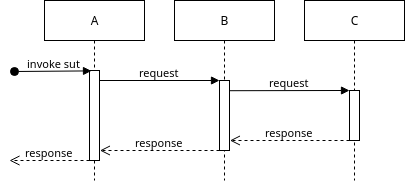
\includegraphics[width=\textwidth]{images/microservice-request-chain.png}
    \caption{Sekvensdiagram der illustrerer hvordan kommunikationskæden mellem microservices}
    \label{fig:microservice-request-chain}
\end{figure}

Problemstillingen her er, at der ikke kan afgrænses et klart test område, da den originale integration test mellem $A$ og $B$, ikke kan kontrollere hvorvidt $B$ kommunikerer med $C$ etc. Dette skyldes netop denne arkitektoniske model, hvor microservices køres som seperate processer og derfor ikke let kan opsættes, så deres eksterne komponenter er opsat med mockede afhængigheder til andre eksterne komponenter. En integration test mellem $A$ og $B$ har derfor mange flere grunde til at fejle, end blot hvorvidt kommunikationen mellem $A$ og $B$ fungerer. Scoped for testen formindskes derfor, så integration tests ikke tager sig af acceptance testing af forretningsopgaven der bedes udført af sammenspillet, men blot kommunikationens succes.

Endnu en af microservicens definerende karakteristika, er autonomi og derigennem selvstændighed: den skal kunne fungere uafhængigt af, om de eksterne komponenter den afhænger af, såsom andre microservices, ikke er tilgængelige. Der skal derfor også eksistere integration tests, der tester på disse scenarier, så det kan garanteres, at selv hvis dens eksterne komponenter er blot delvist utilgængelige, kan dette håndteres således, at den kan give dens minimale funktionalitet.

Integration tests findes i service laget af test pyramiden set i \cref{fig:test-pyramid}. Der skal altså være et mindre antal integration tests end unit tests, men et større antal integration tests end end-to-end tests.

Test af sammenspillet mellem flere microservices, er grundet problemstillingen ved integration tests problematisk. I stedet for, at gå direkte til, at teste sammenspillet mellem flere microservices, giver det derfor mere mening, at man i stedet tester dem isoleret fra hinanden først. Til dette benyttes component testing, om hvilket Martin Fowler siger at ``A component test is a test that limits the scope of the exercised software to a portion of the system under test.'' \footcite{fowler:component-test}

I forbindelse med microservices, giver det perfekt mening, ud fra Fowlers definition, at begrænse scoped for component testing, til en enkelt microservice per component test. Ved at begrænse scopet således, kan forretningsopgaver for en specifik microservices testes i isolation. For at opnå denne isolation, stubbes eksterne komponenter således, at deres opførsel er forudbestemt, så det altid vides hvad der kan forventes af dem. På denne måde, er det nu muligt, at lave letvægtige acceptance tests på et individuelt microservice niveau.

Component tests findes i services laget af test pyramiden set i \cref{fig:test-pyramid}. Der skal altså være et mindre antal component tests end unit tests, men et større antal component tests end end-to-end tests.

Ved brug af unit-, integration og component testing, kan en microservice opnå en god test dækningsgrad i isolation.

\paragraph{Hvordan testes sammenspillet mellem microservices?}\label{sec:how-to-test-microservice-collaboration}

Sammenspillet mellem microservices er, som allerede uddybet i forbindelse med integration testing i \ref{sec:how-to-test-a-microservice}, svært at teste i et afgrænset miljø, grundet microservice arkitekturens natur.

Dette skaber et stort hul i test dækningen af systemet som en samlet helhed, da forventninger mellem kommunikerende microservices, ikke let kan testes i isolation. Der kunne på dette tidspunkt, opsættes en lang række end-to-end tests, der dækker samarbejdet mellem grupper af microservices, men som igen beskrevet i forbindelse med integration testing i \ref{sec:how-to-test-a-microservice}, ville sadanne tests have mange grunde mange flere grunde til at fejle, end blot hvorvidt forventningerne fra en microservice til en anden opfyldes.

Med udgangspunkt i \cref{fig:microservice-request-chain}, ville det altså være mere produktivt, at teste forventningerne en microservice $A$ har til en microservice $B$ i en test, samt forventningerne $B$ har til en microservice $C$ i en anden test.

Konkret er microservices ligeglade med, hvorvidt deres eksterne komponenter opfører sig korrekt og er i stedet kun afhægige af, at de returnerer data som forventet under kommunikationen. Det er derfor fair, at se disse forvetninger om data som resultat af en kommunikation, som værende en kontrakt: microservice $A$ efterspørger en ressource fra microservice $B$; $B$ returnerer ressourcen med de korrekte data tilbage til $A$.

Testning af sadanne kontrakter, er belejligt kaldt contract testing. En contract test tester ikke selve kommunikationsvejene mellem microservices, dette gøres under integration testing som forklaret i \ref{sec:how-to-test-a-microservice}, men blot om de data der returneres under kommunikationen lever op til den kontrakt der eksisterer mellem dem.

Contract tests findes i hvad test pyramiden fra \cref{fig:test-pyramid} kalder "UI" laget - kontrakter kan siges, at danne grænsefladen for en microservice. Der skal altså være et mindre antal contract tests end component/integration tests.

Mens der findes en hvis simplicitet i, at en microservice tester dens egne forventninger til en anden microservice, ville det give mere værdi, at en microservice i stedet tester andre microservices forventninger til den selv. På denne måde, kan summeringen af alle kontrakter til en given microservice benyttes til, at definere de data den faktisk skal returnere, dette er vist i \cref{fig:microservice-contracts}.

\begin{figure}[H]
    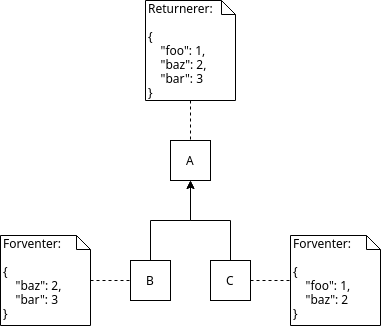
\includegraphics[width=\textwidth]{images/microservice-contracts.png}
    \caption{Illustration af kontrakter mellem microservices}
    \label{fig:microservice-contracts}
\end{figure}

Dette koncept kaldes consumer-driven contracts. Den store fordel ved denne tilgang er, at en microservice nu kan lave regressions testning gennem de contract tests der er defineret til den, således at ændringer i den ikke kan foråsage fejl i andre microservices.

Hvis alle kontrakterne defineret i samtlige microservices contract tests overholdes, kan kommunikationen mellem microservices siges, at være fuldt ud dækket rent test mæssigt. Mens component testing, som beskrevet i \ref{sec:how-to-test-a-microservice}, kan udføre mere letvægtige acceptance tests for microservices i isolation, er der stadig mange forretningsopgaver, der kræver testning af systemet som en helhed.

Sadanne test af systemet som en helhed kaldes end-to-end tests og er allerede nævt flere gange. End-to-end testing dækker alle former for tests, der tester systemet som det bør køre i produktion. I forbindelse med microservices, kunne dette svare til component tests, der ikke benytter sig af stubbede afhængigheder, eller mere klassisk gennem en faktisk grafisk brugergrænseflade.

End-to-end tests findes i toppen af test pyramiden fra \cref{fig:test-pyramid}. Der skal være meget færre end-to-end tests end component/integration tests.

Ved brug af contract- og end-to-end tests, kan sammenspillet og dermed helheden af et system bygget på microservice arkitekturen tests.

\section{Sammenfatning}

Software systemer bygget på microservice arkitekturen, selv med dens lidt særprægede karakteristika, kan på mange måder testes, som man tester et hvilket som helst andet software system. Gennem brug af unit- og component tests, kan individuelle microservices opnå en god test dækningsgrad i isolation. Integration tests garanterer, at kommunikationsveje mellem microservices, både når ting går godt og skidt, fungerer som de skal. Da microservices ikke med lethed kan testes i mindre isolerede grupperinger, testes der i stedet gennem contract tests, på forventningerne mellem microservices hvilke, hvis alle kontrakter overholdes, kan siges at garantere deres funktionalitet i sammenspil. Til sidst benyttes diverse end-to-end tests til, at opnå en mere fyldelsgørende test dækning af systemet som en helhed.

\section{Emner til diskussion}

\begin{itemize}
    \item{Mulighed/nødvendighed for performance testing af sammenspillet mellem microservices.}
    \item{Hvordan opsættes automatiserede test af microservices?}
\end{itemize}

\newpage

\printbibliography

\end{document}

